\documentclass[12pt,titlepage]{article}
\usepackage[dvipsnames,rgb,dvips,table]{xcolor}
\usepackage{graphicx}
\graphicspath{Figures/}
\usepackage{psfrag}
\usepackage{dcolumn}
\usepackage{bm}
\usepackage{amsmath}
\usepackage{amssymb}
\usepackage[rflt]{floatflt}
\usepackage{latexsym}
%\usepackage{float}
\usepackage{bm}
\usepackage{subcaption}
\usepackage{booktabs}
\usepackage{floatrow}
\floatsetup[table]{font=footnotesize}
\usepackage[hidelinks]{hyperref}

%\captionsetup{width=1.1\textwidth}

\usepackage{geometry}
 \geometry{
 left=20mm,
 right=20mm,
 top=25mm,
 bottom=20mm,
 }



%\addtolength{\topmargin}{-1.9cm}
%\addtolength{\textheight}{5.5cm}
%\addtolength{\evensidemargin}{-1.2cm}
%\addtolength{\oddsidemargin}{-1.2cm}
%\addtolength{\textwidth}{2cm}


\pagestyle{myheadings}
\markright{{\small Jacopo Credi  (910216-T396) \,}}
\DeclareMathOperator\erf{erf}
\author{Jacopo Credi \\(910216-T396) \\ \vspace*{2cm} }
\title{{\Large \textsc{Chalmers University of Technology}} \\ \bigskip FFR105 - Stochastic Optimization Algorithms\\ \bigskip Problem set 1 \\ \vspace*{2cm}}

\usepackage{listings}
\usepackage{color} %red, green, blue, yellow, cyan, magenta, black, white
\definecolor{mygreen}{RGB}{28,172,0} % color values Red, Green, Blue
\definecolor{mylilas}{RGB}{170,55,241}
% Settings for writing Matlab code
\lstset{language=Matlab,%
	basicstyle=\small\ttfamily,
    %basicstyle=\color{red},
    breaklines=true,%
    morekeywords={matlab2tikz},
    keywordstyle=\color{blue},%
    morekeywords=[2]{1}, keywordstyle=[2]{\color{black}},
    identifierstyle=\color{black},%
    stringstyle=\color{mylilas},
    commentstyle=\color{mygreen},%
    showstringspaces=false,%without this there will be a symbol in the places where there is a space
    numbers=left,%
    numberstyle={\tiny \color{black}},% size of the numbers
    numbersep=9pt, % this defines how far the numbers are from the text
    %emph=[1]{for,end,break},emphstyle=[1]\color{red}, %some words to emphasise
    frame=single,                   % adds a frame around the code
  	rulecolor=\color{black},
    %emph=[2]{word1,word2}, emphstyle=[2]{style},    
}



\setlength{\parskip}{3pt}
\DeclareMathOperator*{\argmin}{arg\,min}
\usepackage{cases}

\begin{document}
\parindent=0cm
\maketitle

\clearpage\mbox{} \thispagestyle{empty} \clearpage

\section*{Problem 1.1 - Penalty method}
\setcounter{page}{1}
In this problem, we used the penalty method to find the minimum of the function
\begin{equation}
f(x_1,x_2) = (x_1 - 1)^2 + 2(x_2 - 2)^2 \ ,
\end{equation}
subject to the inequality constraint
\begin{equation}
g(x_1,x_2) = x_1^2 + x_2^2 - 1 \leq 0 \ ,
\end{equation}
i.e. $(x_1, x_2)^T \in S, \ $ where $S$ is the unit circle centered at the origin. 

\subsubsection*{(1)}
The penalty function $p(\bm{x} ; \mu)$ of the problem is
\begin{equation}
p(\bm{x} ; \mu) = \mu \Bigl( \max \lbrace g(x_1, x_2), 0 \rbrace \Bigr)^2 = \mu \Bigl( \max \lbrace x_1^2 + x_2^2 - 1, 0 \rbrace \Bigr)^2 \ ,
\end{equation}
thus, the problem can be transformed into an unconstrained minimization of the function
\begin{align}
f_p(\bm{x} ; \mu) =& \ f(x_1,x_2) + p(x_1, x_2 ; \mu) \nonumber \\
=& \ (x_1 - 1)^2 + 2(x_2 - 2)^2 + \mu \Bigl( \max \lbrace x_1^2 + x_2^2 - 1, 0 \rbrace \Bigr)^2 \ .
\end{align}

\subsubsection*{(2)}
The gradient of the function $f_p(\bm{x} ; \mu)$ has a different form, depending on the region where it is calculated:
\[
\underline{\nabla} \ f_p(\bm{x} ; \mu) = \Bigl( \dfrac{\partial f_p}{\partial x_1} , \dfrac{\partial f_p}{\partial x_2} \Bigr)^T \ ,
\]
with
\[
\dfrac{\partial f_p}{\partial x_1} = \begin{cases}
2x_1 - 2 \ , \qquad \qquad  \qquad  \qquad \qquad  \qquad   \text{if} \quad x_1^2 + x_2^2 - 1 \leq 0 \\
2x_1 - 2 + 4\ \mu \ x_1 \ (x_1^2 + x_2^2 - 1) \ , \qquad \text{if} \quad x_1^2 + x_2^2 - 1 > 0 
\end{cases} \ ,
\]
\[
\dfrac{\partial f_p}{\partial x_2} = \begin{cases}
4x_2 -8 \ , \qquad \qquad  \qquad  \qquad \qquad  \qquad   \text{if} \ x_1^2 + x_2^2 - 1 \leq 0 \\
4x_2 -8 +4 \ \mu \ x_2 \ (x_1^2 + x_2^2 - 1) \ , \qquad \text{if} \ x_1^2 + x_2^2 - 1 > 0 
\end{cases} \ .
\]
 
\subsubsection*{(3)}
The unconstrained minimum of $f_p(\bm{x} ; \mu = 0) = f(\bm{x})$ can be found by computing
\[
\underline{\nabla} \ f = 0 \quad \Leftrightarrow \quad \begin{cases} 2x_1 - 2 = 0 \\ 4x_2 - 8 = 0 \end{cases} \quad \Leftrightarrow \quad P_0 = (1, 2)^T \ .
\]
Point $P_0$ is the only stationary point of the function. Let us now compute the eigenvalues of the Hessian matrix $H$, in order to show that the function is convex:
\[
H = 
\begin{pmatrix}
\dfrac{\partial^2 f_p}{\partial x_1^2} & \dfrac{\partial^2 f_p}{\partial x_1 \partial x_2} \\
\dfrac{\partial^2 f_p}{\partial x_2 \partial x_1} & \dfrac{\partial^2 f_p}{\partial x_2^2} \\
 \end{pmatrix} =
 \begin{pmatrix}
2 & 0 \\
0 & 4 \\
 \end{pmatrix} \ .
\]
Since $H$ is diagonal, the diagonal elements are its eigenvalues. They are both positive, so $H$ is positive definite, $f$ is (strictly) convex and since $S$ is a convex set $P_0 = (1, 2)^T$ is the point corresponding to the global minimum. The global minimum of $f$ is therefore $f(1,2) = 0$.

\subsubsection*{(4)}
A \textsc{matlab} program was used to find the minimum of $f_p(\bm{x} ; \mu)$ using the method of gradient descent. The program consists of a main file \texttt{PenaltyMethod.m} which makes use of auxiliary functions \texttt{GradientDescent.m}, \texttt{Gradient.m} and \texttt{FancyPlots.m} and which can be run without requiring any input from the user, i.e. functions $f_p$, $g$, the gradient $\underline{\nabla} \ f_p$ and the parameters needed by the program are hardcoded in the beginning of the main script.

The important parameters of the method are the following:
\begin{itemize}
\setlength\itemsep{-3pt}
\item starting point $\bm{x}_0$ for the gradient descent;
\item sequence of $\mu$ values (\emph{increasing}) for subsequent minimization phases;
\item step length $\eta$ in the gradient descent;
\item threshold value $T$ that determines when to stop the gradient descent.
\end{itemize} 

The program performs a sequence of gradient descents minimizing the function $f_p(\bm{x} ; \mu)$ with increasing $\mu$ (but fixed in each minimization phase) and the output is a $n$-by-3 matrix, where $n$ is the number of $\mu$ values in the input sequence, and where each row $( \mu^{(i)} \ x_1^{*(i)} \ x_2^{*(i)} )$ contains the value taken by $\mu$ in the $i^{th}$ optimization phase and the corresponding position $(x_1^{*(i)}, x_2^{*(i)})$ of the minimum of $f_p$ found in phase $i$.

\subsubsection*{(5)}
The implemented method was applied to minimiz function $f$ in Eq.(1), subject to the inequality constraint in Eq.(2). The unconstrained minimum $P_0$ of $f$ was used as starting point for the first minimization phase, i.e. $\bm{x}_0 = P_0 = (1,2)^T$. The step length was set to $\eta = 10^{-4}$ and the threshold to $T = 10^{-6}$. The used sequence of $\mu$ values is displayed in the first column of Table~\ref{tab::outputTable}, which is exactly the output table produced by the program. The position of the minimum clearly seems to converge to a point on the unit circle, as $\mu$ is increased. 

As shown in Fig.~\ref{fig::11} (left panel), function $f$ evaluations at points found by the program converge to the value -2, which can be claimed to be the solution of the constrained minimization problem. On the right panel, instead, we can see that when $\mu \rightarrow \infty$ the constraint $g(x_1, x_2) \leq 0$ is satisfied.

\begin{table}[H]
\centering
\begin{tabular}{rcc}
\toprule
$\mu$ & $x_1^*$ & $x_2^*$ \\
\midrule
1  &  0.434  &  1.210\\
3   & 0.367 &   1.074\\
10 &   0.331 &   0.996\\
30  &  0.319  &  0.967\\
100 &   0.314 &   0.955\\
300  &  0.312  &  0.952\\
1000  &  0.312  &  0.951\\
\bottomrule
\end{tabular}
\caption{Output table of program \texttt{PenaltyMethod.m} with parameters specified above.}
\label{tab::outputTable}
\end{table}

\begin{figure}[H]
\centering
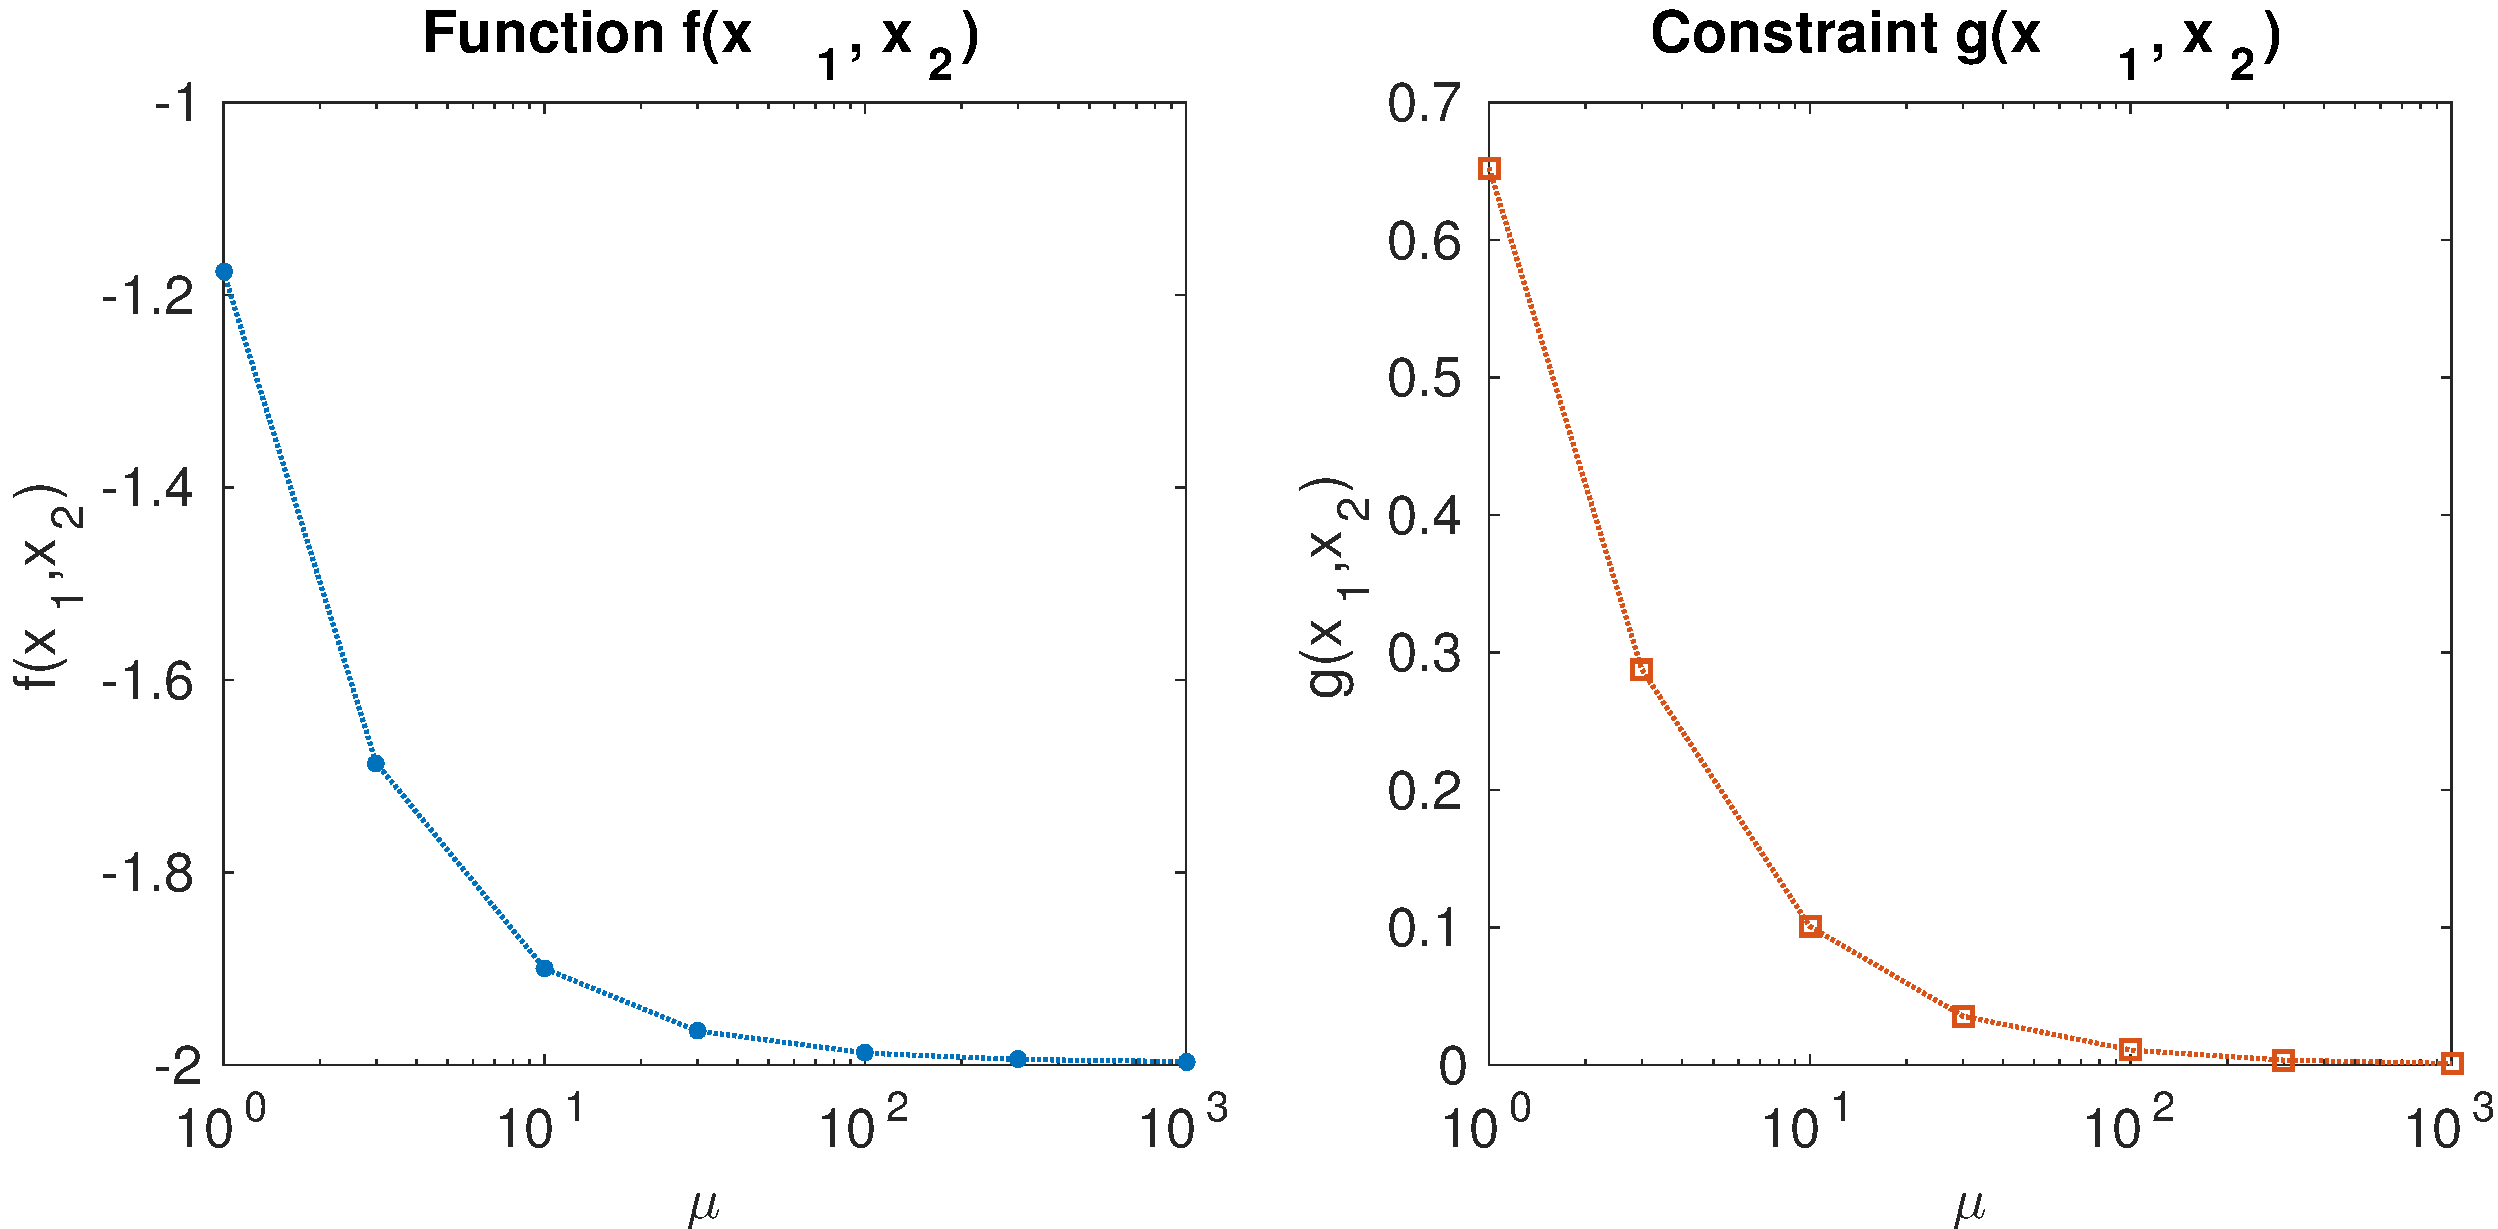
\includegraphics[width=\textwidth]{../Figures/fig11.pdf}
\caption{Functions $f$ (left panel) and $g$ (right panel) evaluated at the points found by the subsequent optimization phases, as $\mu$ is increased.}
\label{fig::11}
\end{figure}


\section*{Problem 1.2 - Constrained optimization}

\subsubsection*{(a)}
Here we are requested to find the global minimum of the function
\begin{equation}
f(x_1, x_2) = 4x_1^2 - x_1 x_2 + 4x_2^2 -6x_2 \ ,
\end{equation}
on the closed set $S$, where $S$ is a triangle with vertices in $A = (0,0)$, $B = (1,1)$, $C = (0,1)$, using the  ``analytical'' method.

\begin{enumerate}
\item \textbf{Find stationary points}
\[
\underline{\nabla} \ f = 0 \ \Leftrightarrow \ \begin{cases} \dfrac{\partial f}{\partial x_1} = 8x_1 -x_2 = 0 \\ \dfrac{\partial f}{\partial x_2} = -x_1 +8x_2 -6 = 0 \end{cases} \Rightarrow \ P_1 = \Bigl(\dfrac{2}{21},\dfrac{16}{21}\Bigr) \ \ \text{is the only stationary point.}
\]
The first critical point to check, $P_1$, lies inside the set $S$.
\item \textbf{Check the boundary $\bm{\partial S}$}
\begin{align*}
x_1 = 0 \ \Rightarrow \ &f(0, x_2) = 4x_2^2 - 6x_2 \\
&\dfrac{\partial}{\partial x_2}f(0, x_2) = 8x_2 - 6 \\
&\dfrac{\partial}{\partial x_2}f(0, x_2^*) = 0 \ \Leftrightarrow \ x_2^* = \dfrac{3}{4} \ \Rightarrow \ P_2 = \Bigl(0, \dfrac{3}{4}\Bigr) \ \text{must also be checked.}
\end{align*}
\begin{align*}
x_2 = 1 \ \Rightarrow \ &f(x_1, 1) = 4x_1^2 - x_1 -2 \\
&\dfrac{\partial}{\partial x_1}f(x_1, 1) = 8x_1 - 1 \\
&\dfrac{\partial}{\partial x_1}f(x_1^*, 1) = 0 \ \Leftrightarrow \ x_1^* = \dfrac{1}{8} \ \Rightarrow \ P_3 = \Bigl(\dfrac{1}{8}, 1\Bigr) \ \text{must also be checked.}
\end{align*}
\begin{align*}
x_1 = x_2 = x \ \Rightarrow \ &f(x, x) = 7x^2 -6x \\
&\dfrac{\partial}{\partial x}f(x, x) = 14x-6 \\
&\dfrac{\partial}{\partial x}f(x^*, x^*) = 0 \ \Leftrightarrow \ x^* = \dfrac{3}{7} \ \Rightarrow \ P_4 = \Bigl(\dfrac{3}{7}, \dfrac{3}{7}\Bigr) \ \text{must also be checked.}
\end{align*}

Also, corners $P_5 = A = (0,0)$, $P_6 = B = (1,1)$, $P_7 = C = (0,1)$ must be checked.

\item \textbf{Evaluate found points one by one}

We have that 
\[
\min\big\lbrace f(P_1), f(P_2), f(P_3), f(P_4), f(P_5), f(P_6), f(P_7) \big\rbrace = f(P_1) = -\dfrac{16}{7} \ ,
\] 
and therefore the global minimum is located in $P_1 = \Bigl(\dfrac{2}{21},\dfrac{16}{21}\Bigr)$.
\end{enumerate}

One could also have computed the eigenvalues of Hessian matrix
\[
H = 
\begin{pmatrix}
\dfrac{\partial^2 f}{\partial x_1^2} & \dfrac{\partial^2 f}{\partial x_1 \partial x_2} \\
\dfrac{\partial^2 f}{\partial x_2 \partial x_1} & \dfrac{\partial^2 f}{\partial x_2^2} \\
 \end{pmatrix} =
 \begin{pmatrix}
8 & -1 \\
-1 & 8 \\
 \end{pmatrix} \ ,
\]
\[
|H-\lambda I_2| = (8-\lambda)^2 -1 = 0 \ \Leftrightarrow \ \lambda_1 = 9, \ \lambda_2 = 7 \ ,
\]
finding that $H$ is positive definite, so the function $f$ is strictly convex and therefore its minimum in the convex set $S$ must be in the interior of $S$ (no need to check the boundary and corners). 

\subsubsection*{(b)}
Here we are requested to find the minimum of the function 
\begin{equation}
f(x_1, x_2) = 15 + 2x_1 + 3x_2 \ ,
\end{equation}
subject to the equality constraint
\begin{equation}
h(x_1, x_2) = x_1^2 + x_1 x_2 +x_2^2 - 21 = 0 \ ,
\end{equation}
using the Lagrange multiplier method.

The Lagrange function $\mathcal{L}(x_1, x_2, \lambda)$ is
\begin{align}
\mathcal{L}(x_1, x_2, \lambda) &= f(x_1, x_2) + \lambda \ h(x_1, x_2) \nonumber \\
&= 15 + 2x_1 + 3x_2 + \lambda \ (x_1^2 + x_1 x_2 +x_2^2 - 21) \ ,
\end{align}
and we have to minimize it with respect to its arguments, by finding stationary points
\begin{numcases}{}
\dfrac{\partial \mathcal{L}}{\partial x_1} = 2 + 2\lambda x_1 + \lambda x_2 = 0 \\
\dfrac{\partial \mathcal{L}}{\partial x_2} = 3 + \lambda x_1 + 2\lambda x_2 = 0 \\
\dfrac{\partial \mathcal{L}}{\partial \lambda} = x_1^2 + x_1 x_2 + x_2^2 - 21 = 0
\end{numcases}
Multiplying Eq.(9) by 2 and subtracting  Eq.(10) from it yields
\begin{equation}
2\times(9) - (10) = 4 + 4\lambda x_1 +2\lambda x_2 - 3 -\lambda x_1 -2\lambda x_2 = 1 + 3\lambda x_1 = 0 \ \Leftrightarrow \ x_1 = -\dfrac{1}{3\lambda} \ .
\end{equation}
Similarly multiplying Eq.(10) by 2 and subtracting Eq.(9) from it yields
\begin{equation}
2\times(10) - (9) = 6 + 2\lambda x_1 +4\lambda x_2 - 2 -2\lambda x_1 -\lambda x_2 = 4 + 3\lambda x_2 = 0 \ \Leftrightarrow \ x_2 = -\dfrac{4}{3\lambda} \ .
\end{equation}
Comparing Eq.(12) and (13) yields $x_2 = 4x_1$, which can be plugged into Eq.(11) to get
\begin{align*}
&x_1^2 + 4x_1^2 + 16x_1^2 = 21 \\
&21x^2 = 21 \ \Leftrightarrow \ x_1 = \pm 1 \ .
\end{align*}
Hence, we obtain two stationary points $P_{1,2} = (\pm 1, \pm 4)$. Clearly, $f(P_1) < f(P_2)$, thus the minimum of $f$ subject to $h = 0$ is $f(P_1) = 1$.

\clearpage
\section*{Problem 1.3 - Basic GA program}

\subsection*{(a)}

A basic genetic algorithm for function optimization was implemented in \textsc{matlab}, starting from the program written during the \textsc{matlab} introduction. The program consists of a main script (\texttt{FunctionOptimization.m}) which calls other functions and which runs without any input, i.e. all parameters are hardcoded in the beginning of the script, whereas the function to minimize is hardcoded in function \texttt{EvaluateIndividual.m}.

An example of the program output on \textsc{matlab} console is displayed in Fig.~\ref{fig::sampleOutput}. At the end of the GA, the program displays the maximum fitness found, the minimum value of the function and its corresponding position. Graphical output, namely the evolution of maximum fitness over the generations and a three-dimensional visualization of the population, is also produced by the program (see e.g. Fig.~\ref{fig::GAtest}).

\begin{figure}[H]
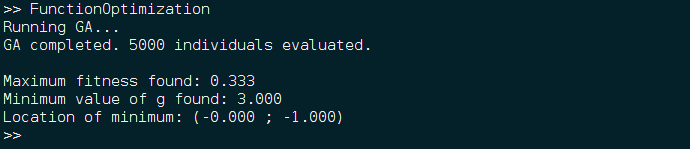
\includegraphics[width=0.7\textwidth]{../Figures/sampleOutput.png}
\caption{Sample console output of the main script \texttt{FunctionOptimization.m}.}
\label{fig::sampleOutput}
\end{figure}


\subsection*{(b)}
The implemented GA optimizer was used to find the (global) minimum value of the function
\begin{align}
g(x_1,x_2) = &\Bigl(1+(x_1 + x_2 + 1)^2(19 - 14x_1 + 3x_1^2-14x_2+6x_1x_2 +3x_2^2)\Bigr) \times \nonumber \\ &\Bigl( 30 + (2x_1-3x_2)^2(18 -32x_1 + 12x_1^2 + 48x_2 -36x_1x_2+27x_2^2)\Bigr)
\end{align}\label{eq::g}in the interval $x_1,x_2 \in [-5,5]$. The fitness function $f$ was defined to be $1/g(x_1,x_2)$.

Each variable $x_i, \ i=1,2$ was encoded with 32 genes/bits ($ m = 64$ is the total chromosome length) and in the elitism step a single copy of the best individual was inserted in the new population at each generation (although the parameter $n_c$ is modifiable in the main script).

After a few test runs, the program was run with the parameters displayed in Table~\ref{tabInitialParams}. Compared to the parameters used in introductory session, the population size was increased to $N = 50$ individuals, and the mutation probability was set to $p_{\textup{mut}} = 1/m$, so that one gene per chromosome is mutated at each step, on average.  The number of generations used in the introductory session ($G = 100$) was estimated to be sufficient and therefore was not changed. 50 runs were performed with these parameters, storing the best solution $(x_1^{\textup{best}}, x_2^{\textup{best}})$ and its fitness value at the end of each run.



\iffalse
The location $(x_1^*, x_2^*)^T$ of the minimum found in this run and the corresponding value of $g$ were 
\[
(x_1^*, x_2^*)^T = (-0.000032, -1.000071)^T \qquad \text{and} \qquad g(x_1,x_2) = 3.000002 \ .
\]
From this first run, we could claim that the true minimum value of $g$ is $3$ and its location is $(0, -1)^T$. Further simulations (see below) indeed supported this claim.
\fi

\begin{table}[H]
\centering
\begin{tabular}{cccccc}
\toprule
Population & Number of & Tournament selection & Tournament  & Crossover  & Mutation \\
size $N$ & generations $G$ & parameter $p_{\textup{tour}}$ & size $j$ & probability	$p_c$ & probability $p_{\textup{mut}}$ \\
\midrule
50 & 100 & 0.75 & 2 & 0.8 & 0.015625\\
\bottomrule
\end{tabular}
\caption{Parameters used for GA optimization.}
\label{tabInitialParams}
\end{table}

\vspace*{-1.1cm}
\begin{figure}[htbp]
\centering
\begin{subfigure}[b]{0.45\textwidth}
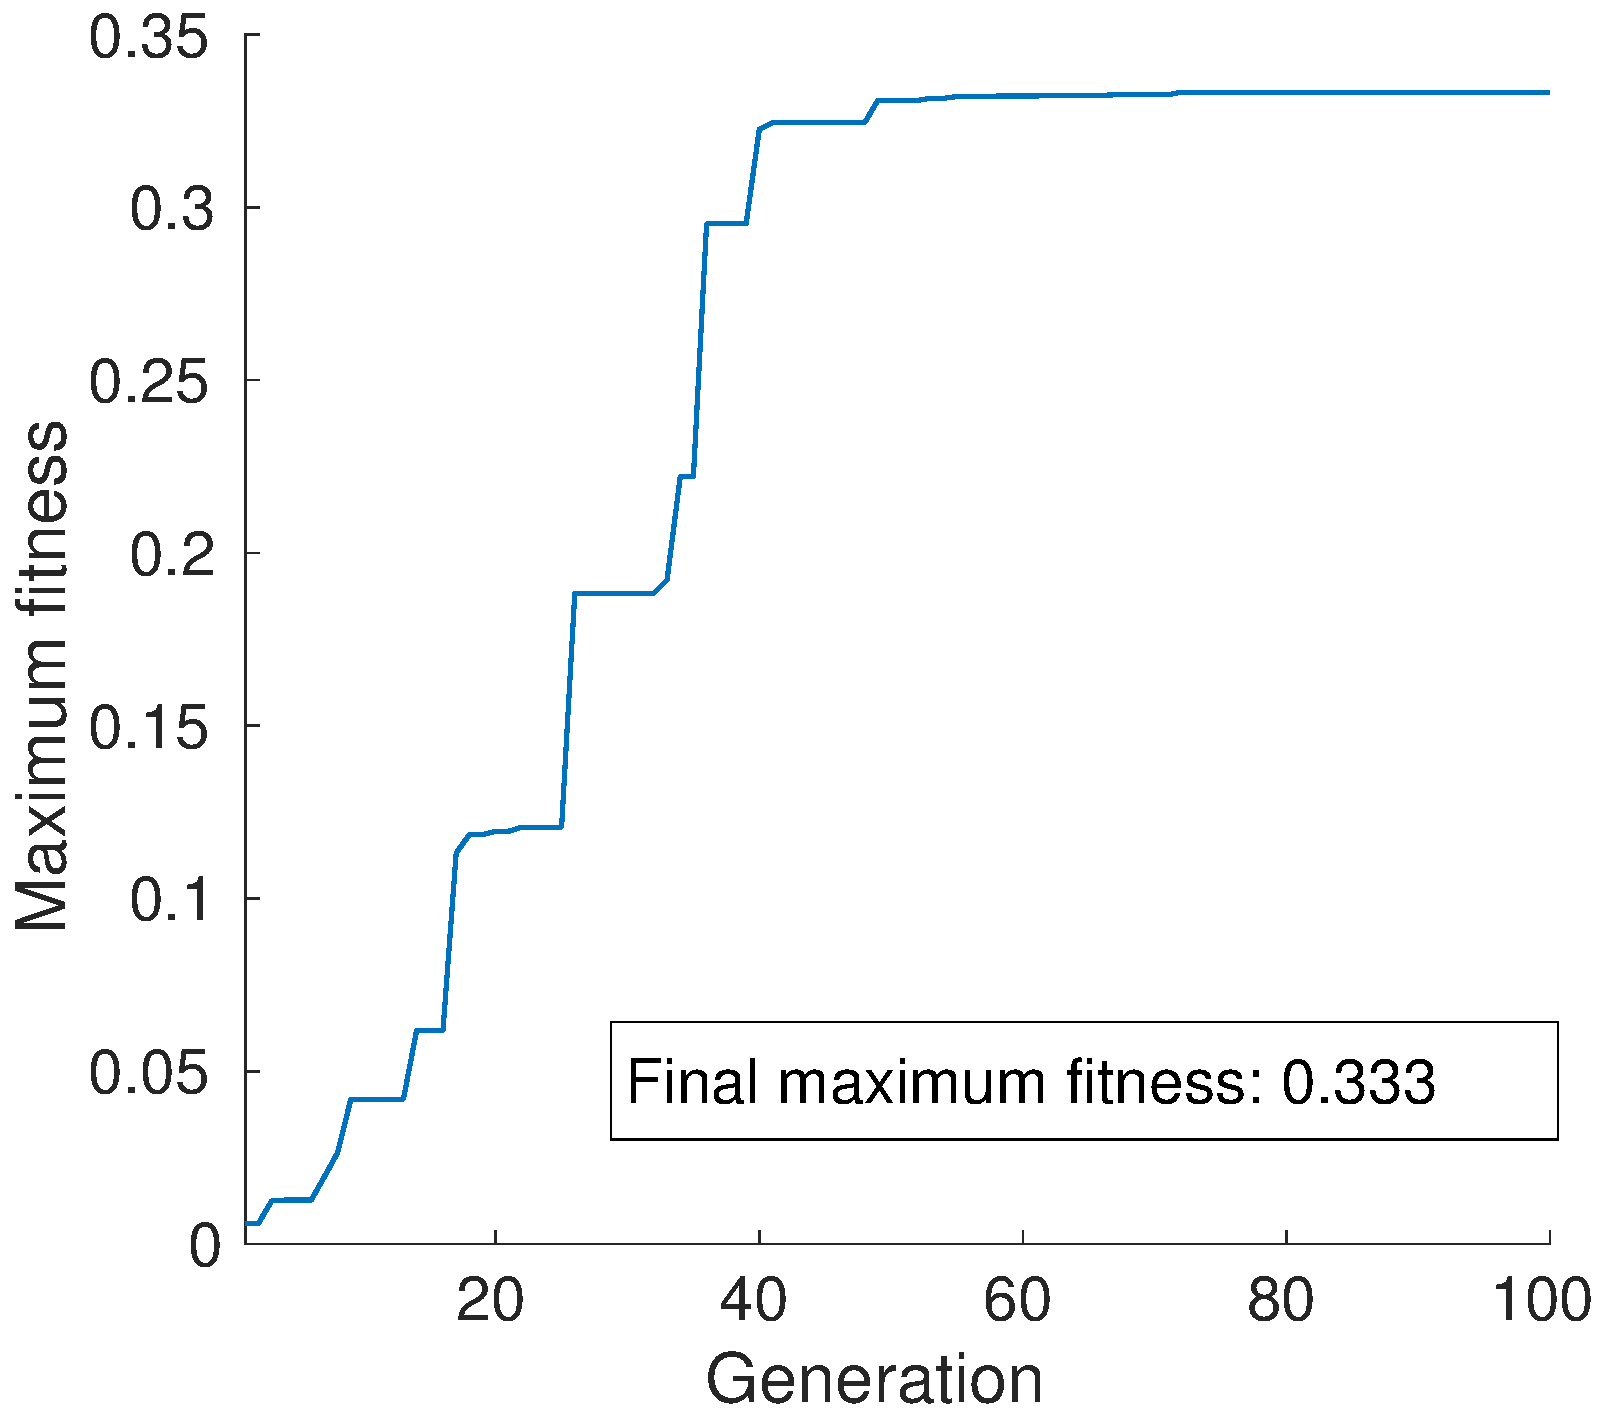
\includegraphics[width=\textwidth]{../Figures/maxFitness.pdf}
\caption{}
\label{subfig::fitnessovertime}
\end{subfigure} \hfill
\begin{subfigure}[b]{0.525\textwidth}
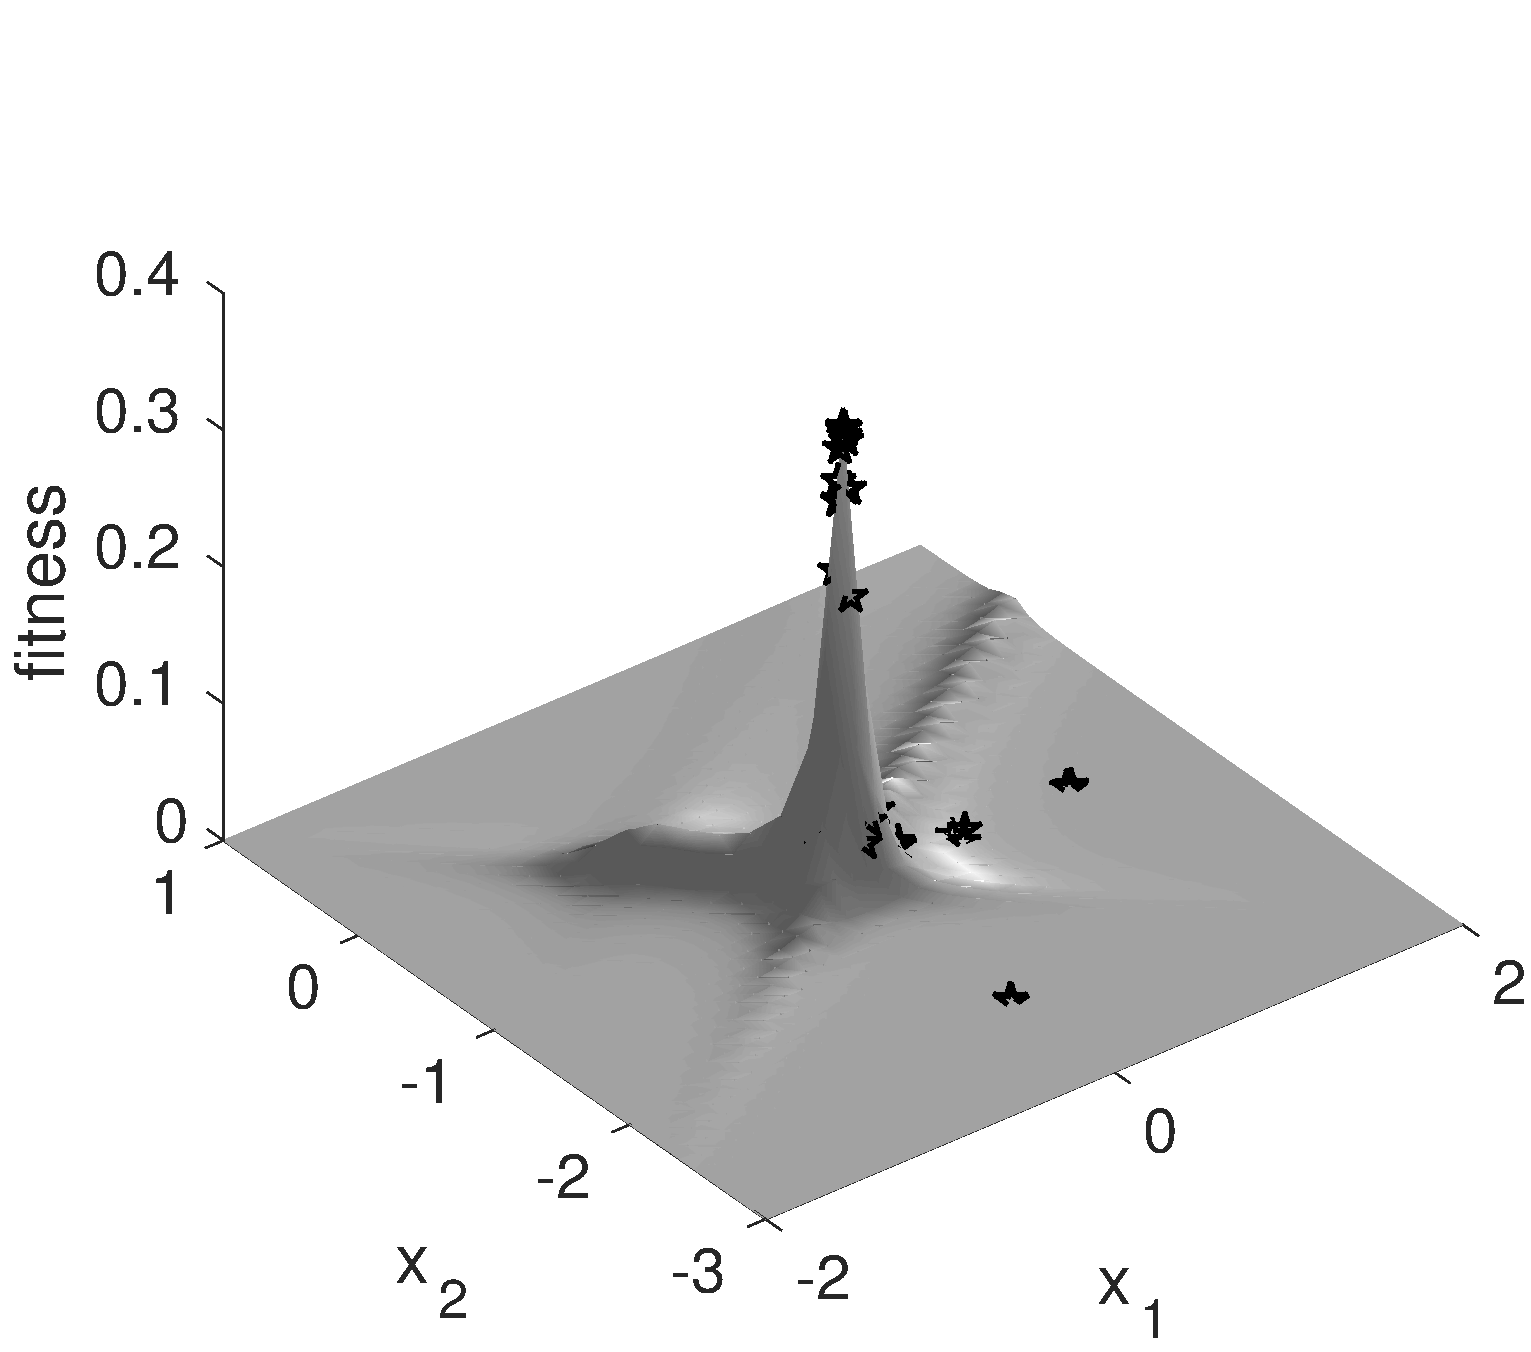
\includegraphics[width=\textwidth]{../Figures/finalPop.pdf}
\caption{}
\label{subfig::finalpop}
\end{subfigure}
\caption{On the left, performance of the GA over time (number of generations). On the right, three-dimensional visualization of the final population in the fitness landscape. Data refers to the last of 50 runs performed with parameters in Table~\ref{tabInitialParams}.} \label{fig::GAtest}
\end{figure}

Fig.~\ref{fig::GAtest}(a) shows the performance (maximum fitness) of the GA as function of time (or, more precisely, of the generation of the solutions population) in the last of these 50 runs. The results obtained by the GA optimizer after this first batch of runs suggest that the (global) minimum value of the function $g$ in the set $S = [-5,5] \times [-5,5]$ and its location are
\[
\min_{(x_1, x_2)^T \in S} g(x_1, x_2) = 3 \qquad \text{and} \qquad \argmin_{(x_1, x_2)^T \in S} g(x_1, x_2) = (0, -1) \ .
\]
We will later see in part \textbf{(c)} that $(0, -1)$ is indeed a stationary point of the function $g$. Table~\ref{tab::basicstats}, instead, displays some basic statistics relative to the set of maximum fitness values $F_{\textup{max}}$ obtained in each run. We will now investigate briefly how changing some of the parameters in Table~\ref{tabInitialParams} affects these statistics.

%\vspace*{-0.1cm}
\begin{table}[H]
\centering
\begin{tabular}{cccc}
\toprule
Sample  & Sample standard & Sample minimum  & Sample maximum \\
mean $\bar{F}_{\textup{max}}$ & deviation $s(F_{\textup{max}})$ & value $\min(F_{\textup{max}})$ & value $\max(F_{\textup{max}})$\\
\midrule
0.295 & 0.090 & 0.012 & 0.333 \\
\bottomrule
\caption{Basic statistics of a sample of 50 values of the maximum fitness obtained at the end of each of 50 runs with parameters in Table~\ref{tabInitialParams}.}
\label{tab::basicstats}
\end{tabular}
\end{table}

\subsubsection*{Effect of selection methods}
The effect of different parameters (tournament selection parameter $p_{\textup{tour}}$ and tournament size $j$) affecting the selection phase was investigated by carrying out 50 runs with different values of $p_{\textup{tour}}$ and $j$ and leaving other parameters unchanged (as in Table~\ref{tabInitialParams}). Maximum fitness statistics in Table~\ref{tab::selection} show that although (at least) one optimal solution is found for each parameter set (see maximum values in the last column), the GA performance decreases as the tournament size is increased from 2 to 5. With such a small population, elitism is probably sufficient to ensure that good solutions survive the selection phase, and large tournaments impair the exploration of new solutions. As for the tournament selection parameter $p_{\textup{tour}}$, its effect is less clear, as the standard deviation of the samples is too high to draw conclusions about it.

\begin{table}[H]
\centering
\begin{tabular}{ccc|cccc}
\toprule
\multicolumn{2}{c}{Selection parameters} & $\quad$ & $\bar{F}_{\textup{max}}$ & $s(F_{\textup{max}})$ & $\min(F_{\textup{max}})$ & $\max(F_{\textup{max}})$ \\
\midrule
$ j = 2$ & $p_{\textup{tour}} = 0.7 $ & & 0.276 & 0.113 & 0.012 & 0.333 \\
$ j = 2$ & $p_{\textup{tour}} = 0.8 $ & & 
0.283 & 0.099 & 0.011 & 0.333 \\
$ j = 2$ & $p_{\textup{tour}} = 0.9 $ & & 0.253 & 0.119 & 0.011 & 0.333 \\
$ j = 5$ & $p_{\textup{tour}} = 0.7 $ & & 0.230 & 0.128 & 0.005 & 0.333 \\
$ j = 5$ & $p_{\textup{tour}} = 0.8 $ & & 0.184 & 0.156 & 0.003 & 0.333 \\
$ j = 5$ & $p_{\textup{tour}} = 0.9 $ & & 0.210 & 0.138 & 0.008 & 0.333 \\
\bottomrule
\caption{Maximum fitness basic statistics for different parameters governing the selection phase of the GA. For other parameters see Table~\ref{tabInitialParams}.}
\label{tab::selection}
\end{tabular}
\end{table}

\subsubsection*{Effect of crossover probability}
The effect of different crossover probabilities $p_c$ was also investigated by carrying out 50 runs with different values of $p_c$ and leaving other parameters unchanged (see Table~\ref{tabInitialParams}). Maximum fitness statistics in Table~\ref{tab::crossover} show that crossover is an important phase allowing the GA to evolve better solutions. In fact, the mean value of the maximum fitness increases monotonically as $p_c$ increases, except for the last case, in which $p_c = 1$. This might suggest that allowing selected individuals to replicate themselves unchanged with a small probability can avoid over-exploitation.

\begin{table}[H]
\centering
\begin{tabular}{cc|cccc}
\toprule
\multicolumn{1}{c}{Crossover probability} & $\quad$ & $\bar{F}_{\textup{max}}$ & $s(F_{\textup{max}})$ & $\min(F_{\textup{max}})$ & $\max(F_{\textup{max}})$ \\
\midrule
$ p_c = 0.00 $ & & 0.286 & 0.084 & 0.012 & 0.333 \\
$ p_c = 0.25 $ & & 0.299 & 0.088 & 0.011 & 0.333 \\
$ p_c = 0.50 $ & & 0.304 & 0.089 & 0.011 & 0.333 \\
$ p_c = 0.80 $ & & 0.304 & 0.079 & 0.011 & 0.333 \\
$ p_c = 0.90 $ & & 0.313 & 0.077 & 0.012 & 0.333 \\
$ p_c = 1.00 $ & & 0.286 & 0.107 & 0.012 & 0.333 \\
\bottomrule
\caption{Maximum fitness basic statistics for different crossover probabilities. For other parameters see Table~\ref{tabInitialParams}.}
\label{tab::crossover}
\end{tabular}
\end{table}

\subsubsection*{Effect of mutation probability}
The effect of different mutation probabilities $p_{\textup{mut}}$ was also investigated by carrying out 50 runs with different values of $p_{\textup{mut}}$ and leaving other parameters unchanged (see Table~\ref{tabInitialParams}). Maximum fitness statistics in Table~\ref{tab::mutation} show that if mutations are completely inhibited the GA performance dramatically drops, as the population is very likely to get stuck in a local optimum. If $p_{\textup{mut}}$ is increased, GA performance gradually increases and reaches its best value for $p_{\textup{mut}} = 3/m$, probably corresponding to a good compromise between exploration and exploitation. Above this value, the excessive randomness seems to negatively affect the GA performance as exploitation is impaired.

\begin{table}[H]
\centering
\begin{tabular}{cc|cccc}
\toprule
\multicolumn{1}{c}{Mutation probability} & $\quad$ & $\bar{F}_{\textup{max}}$ & $s(F_{\textup{max}})$ & $\min(F_{\textup{max}})$ & $\max(F_{\textup{max}})$ \\
\midrule
$ p_{\textup{mut}} = 0 $ & & 0.089 & 0.095 & 0.001 & 0.332 \\
$ p_{\textup{mut}} = 1/2m $ & & 0.251 & 0.112 & 0.011 & 0.333 \\   
$ p_{\textup{mut}} = 1/m $ & & 0.289 & 0.104 & 0.011 & 0.333 \\      
$ p_{\textup{mut}} = 3/m $ & & 0.319 & 0.063 & 0.012 & 0.333 \\
$ p_{\textup{mut}} = 10/m $ & & 0.280 & 0.055 & 0.126 & 0.333 \\
$ p_{\textup{mut}} = 1 $ & & 0.188 & 0.122 & 0.010 & 0.333 \\
\bottomrule
\caption{Maximum fitness basic statistics for different mutation probabilities.}
\label{tab::mutation}
\end{tabular}
\end{table}

\subsection*{(c)}

The point $(x_1^*, x_2^*)^T = (0, -1)^T$ found by the GA can be proven to be a stationary point of the function $g$. Let us first rewrite $g$ as
\begin{align}
g(x_1,x_2) =& \Bigl(1 + \underbrace{(x_1 + x_2 + 1)^2}_{g_1(x_1,x_2)}\underbrace{(19 - 14x_1 + 3x_1^2-14x_2+6x_1x_2 +3x_2^2)}_{g_2(x_1,x_2)}\Bigr) \times \nonumber \\ 
& \Bigl( 30 + \underbrace{(2x_1-3x_2)^2}_{g_3(x_1,x_2)}\underbrace{(18 -32x_1 + 12x_1^2 + 48x_2 -36x_1x_2+27x_2^2)}_{g_4(x_1,x_2)}\Bigr)\nonumber\\
=& \Bigl(1 + g_1(x_1,x_2) g_2(x_1,x_2)\Bigr) \Bigl(30 + g_3(x_1,x_2) g_4(x_1,x_2)\Bigr) \ ,
\end{align} \label{eq::gSimplified}
and note that
\begin{equation}
g_1(x_1^*,x_2^*) = 0 \ , \qquad g_2(x_1^*,x_2^*) = 36 \ , \qquad g_3(x_1^*,x_2^*) = 9 \ , \qquad g_4(x_1^*,x_2^*) = -3 \ .
\end{equation} \label{eq::gValues}Now, by taking the derivative of Eq.(15) with respect to $x_i, \ i=1,2, \ $, we have\footnote{From now on the cumbersome notation $g_j(x_1, x_2)$ is dropped and substituted by $g_j$.}
\begin{align}
\dfrac{\partial g}{\partial x_i} = & \ (30 + g_3 \ g_4) \ \dfrac{\partial}{\partial x_i}(1 + g_1 \ g_2) + (1 + g_1 \ g_2) \ \dfrac{\partial}{\partial x_i} (30 + g_3 \ g_4) \nonumber \\
= & \ (30 + g_3 \ g_4) \Bigl( g_2 \ \dfrac{\partial g_1}{\partial x_i} + g_1 \ \dfrac{\partial g_2}{\partial x_i}\Bigr) + (1 + g_1 \ g_2) \Bigl( g_4 \ \dfrac{\partial g_3}{\partial x_i} + g_3 \ \dfrac{\partial g_4}{\partial x_i} \Bigr)
\end{align} Now, evaluating this generic derivative at point $(x_1^*, x_2^*)^T = (0, -1)^T$ and using values displayed in (16), Eq.(17) simplifies to
\begin{equation}
\dfrac{\partial g}{\partial x_i}\bigg|_{(0,-1)} = 108 \ \dfrac{\partial g_1}{\partial x_i}\bigg|_{(0,-1)} - 3 \ \dfrac{\partial g_3}{\partial x_i}\bigg|_{(0,-1)} + 9 \ \dfrac{\partial g_4}{\partial x_i}\bigg|_{(0,-1)}
\end{equation}

We can now easily compute the derivatives with respect to $x_1$ and $x_2$ and evaluated at $(x_1^*, x_2^*)^T$:
\begin{align*}
\dfrac{\partial g}{\partial x_1}\bigg|_{(0,-1)} &= 216 \ (x_1 + x_2 + 1)\bigg|_{(0,-1)} - 12 \ (2 x_1 - 3x_2)\bigg|_{(0,-1)} + 9 (-32 +24x_1-36x_2)\bigg|_{(0,-1)} \\
&= 0 -36 + 36 \\
&= 0 \ ,
\end{align*}
\begin{align*}
\dfrac{\partial g}{\partial x_2}\bigg|_{(0,-1)} &= 216 \ (x_1 + x_2 + 1)\bigg|_{(0,-1)} + 18 \ (2x_1-3x_2)\bigg|_{(0,-1)} + 9 \ (48 -36x_1 +54x_2)\bigg|_{(0,-1)} \\
&= 0 + 54 - 54 \\
&= 0 \ .
\end{align*}

We have $\underline{\nabla} \ g(0,-1) = (0, 0)^T $, hence the found point is stationary.



\end{document}
